
\chapter{SimSpark and RCSSServer3D}
\label{chSimspark}

This chapter offers a brief introduction of the simulation architecture used in the Robocup 3D Soccer Simulation competitions. The aim of this is to give a global understanding of the inner workings of the system; some details will be skipped, and even then a large part of this information is not necessarily needed to be able to create a team using {\tt libbats}. However, a more fundamental understanding can help a great deal to see what is going on. For a more in-depth treatment, see the SimSpark wiki at \url{http://simspark.sourceforge.net/wiki}.

\section{Basic Architecture}


The RoboCup 3D Soccer Simulation competitions use a unified simulation platform, SimSpark/RCSSServer3D, to supply the simulation of the soccer field, robot mechanics, game rules, etc. In 2006-2007 the first versions of SimSpark were developed, as a generic physics/robotics simulator, with a specific implementation for RoboCup 3D Soccer Simulation. Later on these two parts were explicitly separated: SimSpark now just includes the basic simulation engine, which takes care of the low level physics simulation and interfacing with agents, and exposes several templates to implement specific robot models, visualization systems and a plug-in system. The collection of implementations and plug-ins specific for the RoboCup 3D Simulation league is placed in the separate RCSSServer3D (RoboCup Soccer Simulation Server 3D) package. Together they form what is commonly referred to as '\emph{the simulation server}', '\emph{the simulator}', or '\emph{the server}'.

As said, the simulator takes care of all the world and game aspects. It also supplies a fixed physical robot model, which is the same for each agent an all teams. The simulator determines which sensor information is available for each robot at each time step and executes control commands supplied by the robot's 'brain'. This brain is what a team, i.e. you, has to create in order to be able to participate in the RoboCup 3D Soccer Simulation.

The brain of a robot consists of a standalone program and is connected to its body through a TCP/IP connection; the simulator opens a port (by default 3100), to which your program can connect. After some handshaking messages (explained below), the server will send sensor information at each time step (by default every 0.02 seconds). In reaction to such a sensor message your agent should send a control message, before the end of the time step. This message contains control commands for the agent's controllers, in our case these are target angular velocities for the robot's joints. This perception-action loop is represented in Fig.~\ref{fig:simulator}. This figure also shows that the physics simulation and the visualization of the results of this simulation are separated; the server opens another port (by default 3200), to which a so called '\emph{monitor}' can connect. Through this connection the server sends all information needed by a monitor to make a graphical representation of the current state of the simulation. The monitor in its turn can send commands to the server to control the simulation, which is done for instance when starting the game with a kick off.

\begin{figure}[t]
\begin{center}
	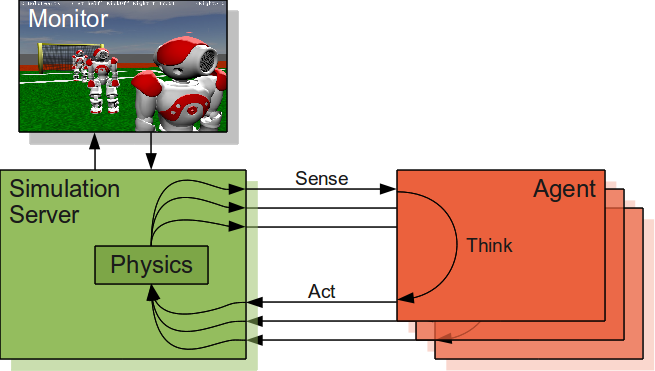
\includegraphics[width=0.70\textwidth]{simulator}
	\captionof{figure}{Interactions between simulator, monitor and agents. Each box represents a stand alone program, arrows between boxes depict the TCP/IP connections used for communication.}
	\label{fig:simulator}
\end{center}
\end{figure}

The communication between the server and the agents and between the server and a monitor follows a Lisp-like protocol, in which messages contain \emph{predicates} in the form of {S-expressions}. A predicate consists of a list of elements, the first of which is the name and the rest are its parameters. These parameters can again be predicates, resulting in a tree of predicates. As a simple example, the statement ``the current game mode number is 6'' is contained in the message {\tt (playMode 6)}. A more extensive example, taken from an actual simulation run, is given in Fig.~\ref{fig:sensemsg}. In the next section we will give an explanation of the different predicates.

\begin{figure}[t]
\begin{center}
\texttt{\small
(\textcolor{Red}{(time (now 70.32))} \textcolor{Blue}{(GS (t 0.00) (pm BeforeKickOff))} \textcolor{Brown}{(GYR (n torso) (rt -0.12 0.13 -0.01))} \textcolor{OliveGreen}{(ACC (n torso) (a -0.06 -0.06 9.81))} \textcolor{Purple}{(HJ (n hj1) (ax 0.00)) (HJ (n hj2) (ax 0.00))} \textcolor{Orange}{(See (G2R (pol 17.64 -12.45 1.00)) (G1R (pol 17.30 -5.75 0.93)) (F1R (pol 17.50 10.54 -1.74)) (F2R (pol 19.35 -26.93 -1.46)) (B (pol 8.69 -18.65 -3.10)) (P (team Enemy) (id 2) (head (pol 15.79 -15.79 0.06)) (rlowerarm (pol 15.75 -15.57 -0.84)) (llowerarm (pol 15.85 -15.84 -0.49)) (rfoot (pol 15.79 -15.37 -1.64)) (lfoot (pol 15.79 -16.08 -1.91))))} \textcolor{Purple}{(HJ (n raj1) (ax 90.00)) (HJ (n raj2) (ax -64.10)) (HJ (n raj3) (ax -0.00)) (HJ (n raj4) (ax -0.03)) (HJ (n laj1) (ax 90.00)) (HJ (n laj2) (ax 64.10)) (HJ (n laj3) (ax -0.00)) (HJ (n laj4) (ax 0.04)) (HJ (n rlj1) (ax 0.01)) (HJ (n rlj2) (ax -0.05)) (HJ (n rlj3) (ax 0.01)) (HJ (n rlj4) (ax -0.00)) (HJ (n rlj5) (ax 0.02)) (FRP (n rf) (c 0.02 -0.03 -0.01) (f 0.19 0.08 21.04)) (HJ (n rlj6) (ax 0.08)) (HJ (n llj1) (ax 0.00)) (HJ (n llj2) (ax 0.01)) (HJ (n llj3) (ax -0.00)) (HJ (n llj4) (ax -0.00)) (HJ (n llj5) (ax 0.03)) (FRP (n lf) (c -0.01 -0.03 -0.02) (f -0.02 0.11 24.22)) (HJ (n llj6) (ax 0.00))})
}
	\captionof{figure}{Example message sent by the server to an agent. Red: time, blue: game state, brown: gyroscopic sensor, green: accelerometer, purple: joint angles, orange: vision.}
	\label{fig:sensemsg}
\end{center}
\end{figure}

\section{Protocol}

Here we will give a small example of a proper communication sequence between an agent and the simulator.

\begin{description}
	\item[Connect] Of course, first of all the agent should connect to the agent port of the server, by default port number 3100.
	\item[Create] After connection, the agent should ask the simulator to create a new robot model for it. This is done with a {\tt scene} predicate, which takes the name of a Ruby Scene Graph (RSG) file that contains the model's description as an argument. Currently, the 3D Simulation League uses a model based on the Nao robot:
	
	{\tt (scene rsg/agent/nao/nao.rsg)}
	\item[Initialize] The server will now start sending messages to the agent. However, before doing anything else, the agent has to finalize its initialization. It has to tell the simulator from which team it is and what uniform number ('\emph{unum}') it wants, by sending an {\tt init} predicate:
	
	{\tt (init (unum 2)(teamname MyTeam))}
	
	If unum 0 is sent, the simulator will appoint the next free uniform number to the agent. In response to this message, the simulator will reply with a message containing confirmation of the uniform number selected by the agent, or chosen by the simulator, and on which side of the field, left or right, the agent's team plays:
	
	{\tt ((time (now 5.80)) \textcolor{Red}{(GS (unum 2) (team left) (t 0.00) (pm BeforeKickOff))} (GYR (n torso) (rt -0.00 0.00 0.00)) (ACC (n torso) (a 0.00 0.00 9.81)) (HJ (n hj1) (ax -0.00))... }
	
	This completes the initial handshake sequence.
	
	\item[Sense] From now on, the simulator sends messages containing time, game state and perceptor information at each time step. You have already seen an example of these in Fig.~\ref{fig:sensemsg}. These senses consist of the state of several internal sensors, namely a gyroscopic and an accelerometric sensor measuring the agen's torso angular velocity and linear acceleration respectively, and two pressure sensors on the feet, and of visual data. This visual data contains the coordinates of objects in the field of view of the agent, i.e. the ball, several body parts of other agents, corner flags and goal posts, and lines. The field of view of an agent is by default 120 degrees both horizontally as vertically.
	
	\item[Act] After each simulator message, the agent should reply with an action message. Such a message contains control commands for the agent's actuators, i.e. a target angular velocity for each joint. For instance, the following message tells the simulator to move the two head joints {\tt he1} and {\tt he2}, and the first joints of both arms, {\tt lae1} and {\tt rae2}\footnote{SimSpark's communication protocol measures angles in degrees. Note however that {\tt libbats} internally uses radians, (and radians per second for angular velocities).}:
	
	{\tt (he1 11.759) (he2 -8.4038) (lae1 -18.987) (rae1 -18.985)}
	
	If for some joints no control is specified, the last target angular velocity that was sent is used by the simulator. Besides the joint actuators, there is a special 'beam' actuator, that can be used to quickly position an agent before kick-offs. It takes as arguments the x and y coordinates to beam to and the angle to face at. So, to beam to coordinates (-7, 1.5), while face angle 0, which is towards the opponent's goal, the agent should send the following message:
	
	{\tt (beam -7 1.5 0)}
	
\end{description}

%\section{Robot Model}

%The agent model used in the RoboCup 3D Soccer Simulation competitions is of a humanoid robot, roughly based on Aldeberan's Nao robot, shown 
